\documentclass{scrartcl}
\usepackage[utf8]{inputenc} 
\usepackage[T1]{fontenc} 
\usepackage[dvipsnames]{xcolor} 
\usepackage[object=vectorian]{pgfornament}   
\usetikzlibrary{shapes.geometric,calc}
\definecolor{fondpaille}{cmyk}{0,0,0.1,0}
\begin{document}
\pagecolor{fondpaille}
\color{Maroon}   

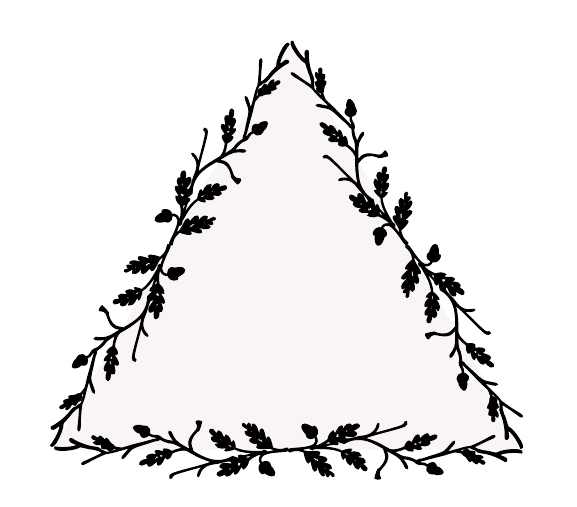
\begin{tikzpicture}
\node (A) at (0,0) {};  
\node (B) at (0:6) {};  
\node (C) at (60:6) {}; 
\path [fill=Maroon!10,fill opacity=.4,text opacity=1]     
 (A.center) to [ornament=87] (B.center) to [ornament=87] 
 (C.center) to [ornament=87] (A.center);
\end{tikzpicture}      
\end{document}  


                       